
\iffalse
\documentclass[journal,12pt,twocolumn]{IEEEtran}
\usepackage{cite}
\usepackage{amsmath,amssymb,amsfonts,amsthm}
\usepackage{algorithmic}
\usepackage{graphicx}
\usepackage{textcomp}
\usepackage{xcolor}
\usepackage{txfonts}
\usepackage{listings}
\usepackage{enumitem}
\usepackage{mathtools}
\usepackage{float}
\usepackage{gensymb}
\usepackage{comment}
\usepackage[breaklinks=true]{hyperref}
\usepackage{tkz-euclide} 
\usepackage{listings}
\usepackage{gvv}                                        
\def\inputGnumericTable{}                                 
\usepackage[latin1]{inputenc}                                
\usepackage{color}                                            
\usepackage{array}                                            
\usepackage{longtable}                                       
\usepackage{calc}                                             
\usepackage{multirow}                                         
\usepackage{hhline}                                           
\usepackage{ifthen}                                           
\usepackage{lscape}
\usepackage{amsmath}
\newtheorem{theorem}{Theorem}[section]
\newtheorem{problem}{Problem}
\newtheorem{proposition}{Proposition}[section]
\newtheorem{lemma}{Lemma}[section]
\newtheorem{corollary}[theorem]{Corollary}
\newtheorem{example}{Example}[section]
\newtheorem{definition}[problem]{Definition}
\newcommand{\BEQA}{\begin{eqnarray}}
\newcommand{\EEQA}{\end{eqnarray}}
\newcommand{\define}{\stackrel{\triangle}{=}}
\theoremstyle{remark}
\newtheorem{rem}{Remark}

\begin{document}

\bibliographystyle{IEEEtran}
\vspace{3cm}

\title{NCERT Discrete - 11.9.1.8}
\author{EE23BTECH11045 - Palavelli Srija$^{*}$}

\maketitle
\newpage
\bigskip

\renewcommand{\thefigure}{\theenumi}
\renewcommand{\thetable}{\theenumi}

\vspace{3cm}
\textbf{Question 11.9.1.8:} 
\begin{enumerate}
\item Find the seventh term of the sequence where the nth term is given by $a_n= \frac {n^2}{2^{n}}$
\end{enumerate}

\textbf{Solution: }
\fi
\begin{align}
 x(n) &= \frac{(n+1)^2}{2^{(n+1)}}u(n)
\end{align}

\begin{table}[h!]
    \centering
     \begin{tabular}{|c|c|}
        \hline
        \textbf{Parameter} & \textbf{Value} \\
        \hline
        \(x(n)\) & \(\frac{(n+1)^2}{2^(n+1)}u(n)\) \\ \\
        \(x(6)\) & ? \\
        \hline
    \end{tabular}

    \caption{Input Parameters}
    \label{tab:table_9.8.1}
\end{table}

\begin{align}
x(6) &= \frac{(6+1)^2}{2^{(6+1)}}\\
     &= \frac {49}{128}
\end{align}

\begin{enumerate}
   \item Scaling property:
     \begin{align}
         a^{n} u(n) & \xleftrightarrow{\mathcal{Z}}  \frac{1}{(1-az^{-1})}, \quad \lvert z \rvert > \lvert a \rvert 
     \end{align}
     
   \item Differentiation property:
    \begin{align}
     n u(n) & \xleftrightarrow{\mathcal{Z}} (-z) \frac{dY(z)}{dz} \\
     \implies n u(n) & \xleftrightarrow{\mathcal{Z}}  \frac{z^{-1}}{(1-z^{-1})^2}, \quad \lvert z \rvert > 1 \\
     \implies n^2 u(n) & \xleftrightarrow{\mathcal{Z}}  \frac{z^{-1}(1+z^{-1})}{(1-z^{-1})^3}, \quad \lvert z \rvert > 1
   \end{align}
   
   \item Time shifting property:
    \begin{align}
         y(n-k) & \xleftrightarrow{\mathcal{Z}} z^{-k}Y(z)
     \end{align}
\end{enumerate}

The Z transform of $x(n)$ is given by:\\
from(4)
\begin{align}
\frac{u(n)}{2^n} & \xleftrightarrow{\mathcal{Z}}  \frac{1}{(1-(2z)^{-1})}, \quad \lvert z \rvert>\frac{1}{2}
\end{align}
	from(5)
\begin{align}
\frac{n}{2^n} u(n) & \xleftrightarrow{\mathcal{Z}} \frac{(2z)^{-1}}{(1-(2z)^{-1})^2}, \quad \lvert z \rvert>\frac{1}{2}\\
\frac{n^2}{2^n} u(n) & \xleftrightarrow{\mathcal{Z}} \frac{(2z)^{-1}(1 + (2z)^{-1})}{(1 - (2z)^{-1})^3}, \quad \lvert z \rvert>\frac{1}{2}
\end{align}
	from(8)
\begin{align}
\frac{(n+1)^2}{2^(n+1)} u(n) & \xleftrightarrow{\mathcal{Z}} (z) \frac{(2z)^{-1}(1 + (2z)^{-1})}{(1 - (2z)^{-1})^3}, \quad \lvert z \rvert > \frac{1}{2}
\end{align}

\begin{align}
X(z) &= \frac{1 + (2z)^{-1}}{2(1 - (2z)^{-1})^3}, \quad \lvert z \rvert > \frac{1}{2}
\end{align}

\begin{figure}[h!]
    \centering
    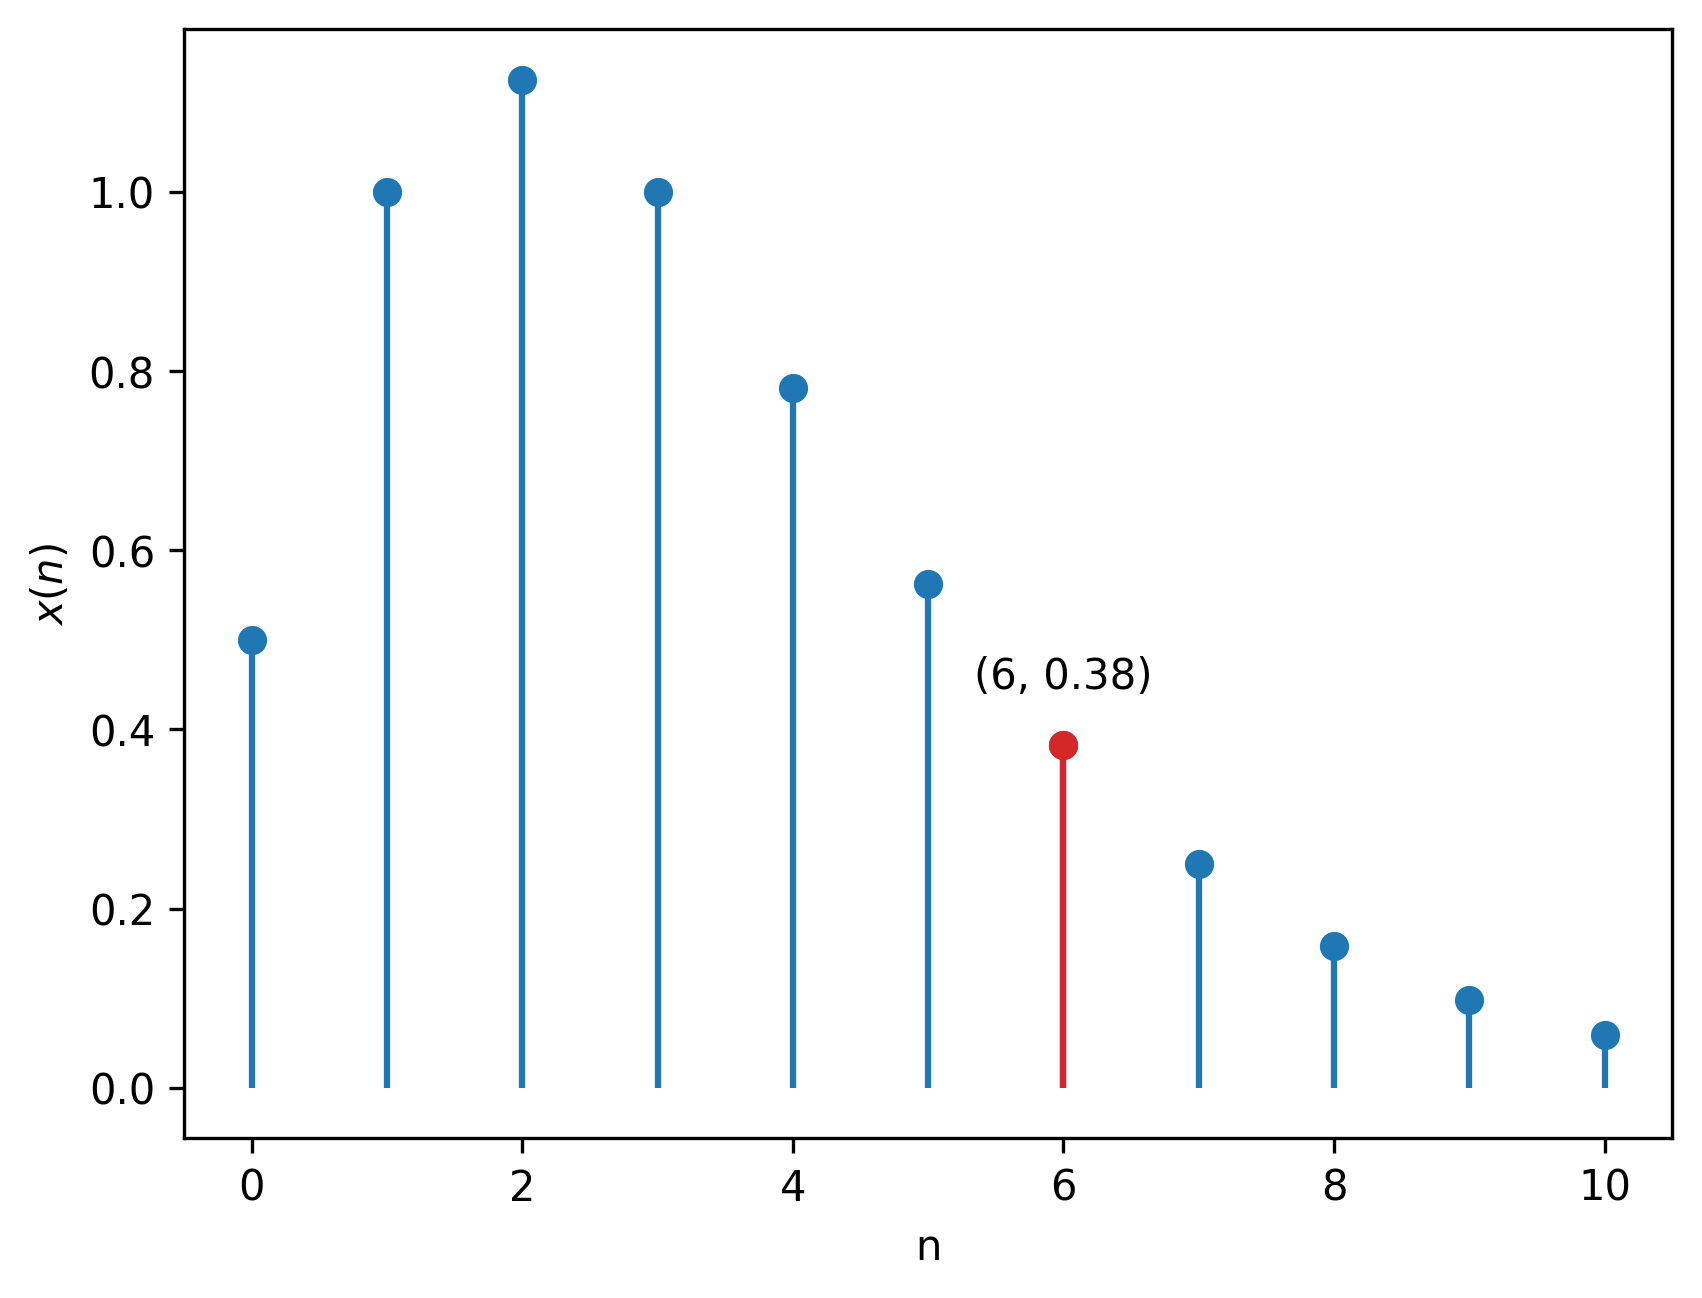
\includegraphics[width=\columnwidth]{ncert-maths/11/9/1/8/figs/plot.png}
    \caption{Stem plot of $x(n)$}
    \label{fig:1}
\end{figure}

%\end{document}
